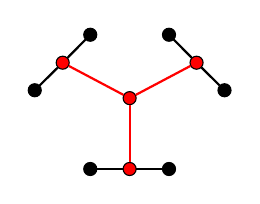
\begin{tikzpicture}[auto,scale=0.5]

	\node (c0) [circle, draw, fill=black, scale=0.5] at (0, 0) {};
	\node (c1) [circle, draw, fill=black, scale=0.5] at (2, 0) {};
	\node (c2) [circle, draw, fill=black, scale=0.5] at (0, 3.41) {};
	\node (c3) [circle, draw, fill=black, scale=0.5] at (-1.41, 2) {};
	\node (c4) [circle, draw, fill=black, scale=0.5] at (2, 3.41) {};
	\node (c5) [circle, draw, fill=black, scale=0.5] at (3.41, 2) {};
	\node (c6) [circle, draw, fill=red, scale=0.5] at (1, 0) {};
	\node (c7) [circle, draw, fill=red, scale=0.5] at (-0.7, 2.7) {};
	\node (c8) [circle, draw, fill=red, scale=0.5] at (2.7, 2.7) {};
	\node (c9) [circle, draw, fill=red, scale=0.5] at (1, 1.8) {};

	\path[thick]
	(c0) edge (c6)
	(c6) edge (c1)
	(c2) edge (c7)
	(c7) edge (c3)
	(c4) edge (c8)
	(c8) edge (c5)
	(c6) edge[red] (c9)
	(c7) edge[red] (c9)
	(c8) edge[red] (c9);

\end{tikzpicture}
